

\chapter{EXPERIMENT 4: AN INVESTIGATION OF THE REGISTER} \label{ap:exp4}

One alternative hypothesis that might explain the present agreement attraction in Turkish is the honorific interpretation of the \emph{-lar} marking on the verb. As discussed in Chapter \ref{ch:intro}, plural marking on the verb does not necessarily mean the subject is plural. In some instances, it is a morphological reflex of the formal register in Turkish. This additional meaning of the \emph{-lar} marking raised the following question: `Can attraction effects arise in informal registers?' If the hypothesis mentioned above is the underlying reason for the attraction effect, we would expect no effect of plural attractor in ungrammatical sentences when we have an informal setting. To this end, we modified our experimental sentences from Experiment 1. We included a new register manipulation with two factors: a formal register with a post-verbal \emph{efendim} (\emph{sir}) and an informal register with a post-verbal \emph{lan} (\emph{yo}). 

\section{Participants}
Our participants (N = 174) were native Turkish speakers and Bo\u{g}azi\c{c}i University undergraduate students. In exchange for attending the experiment, they were given extra credit in one of the pre-determined Linguistics courses. The average age of participants was 21, ranging from 18 to 59. In the experimental process, both the principles of the Declaration of Helsinki and the regulations concerning research ethics at Bo\u{g}azi\c{c}i University were followed without any exception. Before the experiment, all participants were asked to provide informed consent. During the experiment, any information regarding their identities was not collected. 

\section{Materials}

In Experiment 4, we used the same 40 items from Experiment 1, but we included another manipulation. In addition to manipulating the number of the verb and the attractor (singular x plural), we also manipulated the register of the item (formal x informal). We added a post-verbal interjection in all experiment items. The formal register conditions had an interjection which can be translated as \emph{sir}. In contrast, the informal register conditions ended with an interjection like \emph{yo} or dude. One set of experimental conditions can be found in (\ref{ex:exp4items}). One thing to note in these conditions is that the presence of a plural verb creates ungrammaticality only in informal registers. There is a speaker variability in the use of -lar as a formal register marker: while to some Turkish speakers, the word sir licenses the plural marker, for some, it does not. We showed this variability with the \% symbol.


\ea \label{ex:exp4items}
    \ea {Informal Register}
        \ea[*]{{Plural Attractor, Plural Verb} \label{ex:exp4-informal-plpl}\\*
        \gll [Milyoner-ler-in {terzi-si}] tamamen gereksizce {kov-ul-du-lar} lan.\\
        millionaire-\Pl-\Gen{} tailor-\Poss{} completely without.reason fire-\Pass-\Pst-\Tpl{} yo\\
        \glt `Yo, the millionaires' tailor were fired for no reason at all.'}
        \ex[]{{Plural Attractor, Singular Verb} \label{ex:exp4-informal-plsg} \\*
        \gll [Milyoner-ler-in {terzi-si}] tamamen gereksizce {kov-ul-du} lan.\\
        millionaire-\Pl-\Gen{} tailor-\Poss{} completely without.reason fire-\Pass-\Pst{} yo\\
        \glt `Yo, the millionaires' tailor was fired for no reason at all.'}
        \ex[*]{{Singular Attractor, Plural Verb} \label{ex:exp4-informal-sgpl}\\*
        \gll [Milyoner-in {terzi-si}] tamamen gereksizce {kov-ul-du-lar} lan.\\
        millionaire-\Gen.\Sg{} tailor-\Poss{} completely without.reason fire-\Pass-\Pst-\Tpl{} yo\\
        \glt `Yo, the millionaire's tailor were fired for no reason at all.'}
        \ex[]{{Singular Attractor, Singular Verb} \label{ex:exp4-informal-sgsg}\\*
        \gll [Milyoner-in {terzi-si}] tamamen gereksizce {kov-ul-du} lan.\\
        millionaire-\Gen.\Sg{} tailor-\Poss{} completely without.reason fire-\Pass-\Pst{} yo\\
        \glt `Yo, the millionaire's tailor was fired for no reason at all.'}
        \z
    \ex {Formal Register}
        \ea[\%]{{Plural Attractor, Plural Verb} \label{ex:exp4-formal-plpl}\\*
        \gll [Milyoner-ler-in {terzi-si}] tamamen gereksizce {kov-ul-du-lar} efendi-m.\\
        millionaire-\Pl-\Gen{} tailor-\Poss{} completely without.reason fire-\Pass-\Pst-\Tpl{} sir-\Fsg.\Poss{}\\
        \glt `Sir, the millionaires' tailor were fired for no reason at all.'}
        \ex[]{{Plural Attractor, Singular Verb} \label{ex:exp4-formal-plsg} \\*
        \gll [Milyoner-ler-in {terzi-si}] tamamen gereksizce {kov-ul-du} efendi-m.\\
        millionaire-\Pl-\Gen{} tailor-\Poss{} completely without.reason fire-\Pass-\Pst{} sir-\Fsg.\Poss{}\\
        \glt `Sir, the millionaires' tailor was fired for no reason at all.'}
        \ex[\%]{{Singular Attractor, Plural Verb} \label{ex:exp4-formal-sgpl}\\*
        \gll [Milyoner-in {terzi-si}] tamamen gereksizce {kov-ul-du-lar} efendi-m.\\
        millionaire-\Gen.\Sg{} tailor-\Poss{} completely without.reason fire-\Pass-\Pst-\Tpl{} sir-\Fsg.\Poss{}\\
        \glt `Sir, the millionaire's tailor were fired for no reason at all.'}
        \ex[]{{Singular Attractor, Singular Verb} \label{ex:exp4-formal-sgsg}\\*
        \gll [Milyoner-in {terzi-si}] tamamen gereksizce {kov-ul-du} efendi-m.\\
        millionaire-\Gen.\Sg{} tailor-\Poss{} completely without.reason fire-\Pass-\Pst{} sir-\Fsg.\Poss{}\\
        \glt `Sir, the millionaire's tailor was fired for no reason at all.'}
        \z
    \z
\z

The experiment also included two sub-experiments in it, which served as fillers. The first sub-experiment was concerned with the suspended affixation and manipulated the presence of suspended affixation (no SA x SA) and the type of the conjoiner (ve x ya da). Our experiment included 40 items with four conditions as in (\ref{ex:sa-sub}). 

\ea \label{ex:sa-sub}
    \ea[]{{And Conjoiner, No Suspended Affixation}\\*
    \gll De-di\u{g}-in-e g\"ore bana ve Furkan-a izin ver-ecek.\\
    say-\Nmlz-\Poss-\Dat{} according\_to I.\Dat{} and Furkan-\Dat{} permission grant-\Fut{}\\
    \glt `According to what she said, she will grant permission to me and Furkan.'}
    \ex[]{{Or Conjoiner, No Suspended Affixation}\\*
    \gll De-di\u{g}-in-e g\"ore bana {ya da} Furkan-a izin ver-ecek.\\
    say-\Nmlz-\Poss-\Dat{} according\_to I.\Dat{} or Furkan-\Dat{} permission grant-\Fut{}\\
    \glt `According to what she said, she will grant permission to me or Furkan.'}
    \ex[\%]{{And Conjoiner, Suspended Affixation}\\*
    \gll De-di\u{g}-in-e g\"ore ben ve Furkan-a izin ver-ecek.\\
    say-\Nmlz-\Poss-\Dat{} according\_to I and Furkan-\Dat{} permission grant-\Fut{}\\
    \glt `According to what she said, she will grant permission to me and Furkan.'}
    \ex[\%]{{Or Conjoiner, Suspended Affixation}\\*
    \gll De-di\u{g}-in-e g\"ore ben {ya da} Furkan-a izin ver-ecek.\\
    say-\Nmlz-\Poss-\Dat{} according\_to I or Furkan-\Dat{} permission grant-\Fut{}\\
    \glt `According to what she said, she will grant permission to me or Furkan.'}
    \z
\z

The other sub-experiment was concerned with the relationship between suspended affixation and the type of embedded clause that encompasses the suspended affixation. The sub-experiment manipulated the presence of suspended affixation (SA x no SA) and the embedded clause type (conditional x temporal adverbial). Our experiment included 40 items with four conditions as in (\ref{ex:sa-cond}). 


\ea \label{ex:sa-cond}
    \ea[]{{Conditional, No Suspended Affixation}\\*
    \gll E\u{g}er yaz{\i}n k\"oy-e veya tatil-e gid-ebil-ir-se-m \c{c}ok e\u{g}len-iyor-um.\\
    if in\_summers village-\Dat{} or vacation-\Dat{} go-\Abil-\Aor-\Cond-\Fpl{} very have\_fun-\Impf-\Fpl{}\\
    \glt `If I can go to the village or a vacation in summers, I have so much fun.'}
    \ex[]{{Conditional, Suspended Affixation}\\*
    \gll E\u{g}er yaz{\i}n k\"oy veya tatil-e gid-ebil-ir-se-m \c{c}ok e\u{g}len-iyor-um.\\
    if in\_summers village or vacation-\Dat{} go-\Abil-\Aor-\Cond-\Fpl{} very have\_fun-\Impf-\Fpl{}\\
    \glt `If I can go to the village or a vacation in summers, I have so much fun.'}
    \ex[]{{Temporal Adverbial, No Suspended Affixation}\\*
    \gll Yaz{\i}n k\"oy-e veya tatil-e gid-ebil-ince \c{c}ok e\u{g}len-iyor-um.\\
    in\_summers village-\Dat{} or vacation-\Dat{} go-\Abil-\When{} very have\_fun-\Impf-\Fpl{}\\
    \glt `When I get go to the village or a vacation in summers, I have so much fun.'}
    \ex[]{{Temporal Adverbial, Suspended Affixation}\\*
    \gll Yaz{\i}n k\"oy veya tatil-e gid-ebil-ince \c{c}ok e\u{g}len-iyor-um.\\
    in\_summers village or vacation-\Dat{} go-\Abil-\When{} very have\_fun-\Impf-\Fpl{}\\
    \glt `When I get to go to the village or a vacation in summers, I have so much fun.'}
    \z
\z

All of our experimental and filler items can be found in Appendix \ref{ap:exp4items}

\section{Procedure}

Experiment 4 was carried out in the same manner as Experiment 1. However, participants had 40 experimental items and 80 fillers, coming from two sub-experiments. Participants did not see all conditions from these sub-experiments since they were also distributed among four different lists. Since there are no real fillers, we believe this experiment should be replicated in a proper experimental setting without sub-experiments. However, we also think that the presence of 80 agreement attraction irrelevant items would make participants pay less attention to attraction items. 

\section{Analysis}

In Experiment 4, we only removed participants according to their accuracy in practice items. We excluded 8 participants from our experiments who answered more than half of the practice items wrong.

We analyzed yes responses with a Bayesian Generalized Linear Model in which we assumed that responses were distributed following a Bernoulli distribution with a probit link function. Furthermore, we analyzed only experimental sentences without including the missing data in the formula and used three categorical predictors and their interactions. We used (i) verb number, (ii) attractor number, and (iii) formal register, as well as their interactions as predictors. Moreover, we used by-participant and by-item intercepts and slopes for all predictors. All factors were sum-coded. We used 0.5 for the following levels: (i) plural verb, (ii) plural attractor, and (iii) formal register. 

We have used the same priors that were specified in the analysis of Experiment 1. 

\section{Results}

Figure \ref{fig:exp4AvgResponse} shows the average proportions of acceptable responses by experimental conditions for Experiment 4. The x-axis shows the register type (formal x informal), and the y-axis shows the percentage `acceptable'. The line type represents the attractor number. The dotted lines signal singular attractors, and the solid lines signal plural attractors. The graph has two facets: Singular verbs on the left-hand side and plural verbs on the right-hand side.

\begin{knitrout}
\definecolor{shadecolor}{rgb}{0.969, 0.969, 0.969}\color{fgcolor}\begin{figure}[hbt!]

{\centering 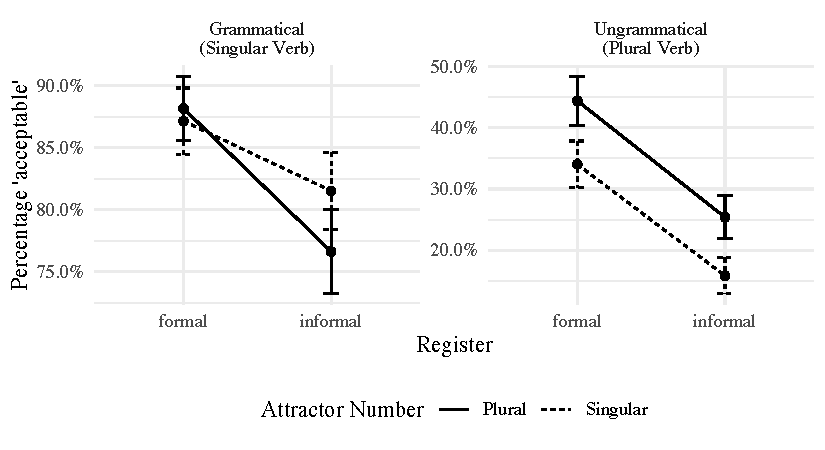
\includegraphics[width=\linewidth]{figure/exp4AvgResponse-1} 

}

\caption{The average percentage of acceptable responses according to the experimental conditions in Experiment 4}\label{fig:exp4AvgResponse}
\end{figure}

\end{knitrout}

We see that in both formal and informal registers, participants accepted sentences with plural attractor and verb (M = 0.44 and 0.25, SE = 0.02 and 0.02, for formal and informal registers, respectively) more often than singular attractor counterparts (M = 0.34 and 0.16, SE = 0.02 and 0.02, for formal and informal registers, respectively). This clearly shows that the agreement attraction effects were due to a possible honorific reading. 

As we expected, formal registers with words like \emph{sir} licensed the presence of a plural verbal agreement. However, due to the speaker variability, the acceptability of sentences with a plural verb in the formal register conditions (M = 0.44 and 0.34, SE = 0.02 and 0.02, for singular and plural attractor conditions, respectively) were not on par with the sentences with the singular verb in the formal register conditions (M = 0.88 and 0.87, SE = 0.01 and 0.01, for singular and plural attractor conditions, respectively). Interestingly, in informal registers, there is a slight difference between singular attractor (M = 0.82, SE = 0.02) and plural attractor conditions (M = 0.77, SE = 0.02) with plural verb. We also see that singular verbs in informal registers were accepted less often than those in the formal register conditions. 

Figure \ref{fig:exp4Bayes} shows the coefficient posterior summaries extracted from our Bayesian GLM fitted to the data from Experiment 4. On the right-hand side, we see the posterior probability of the effect of a coefficient being smaller than 0. The dot shows the mean estimate of the posteriors while the line indicates 95\% credible intervals.

\begin{knitrout}
\definecolor{shadecolor}{rgb}{0.969, 0.969, 0.969}\color{fgcolor}\begin{figure}[hbt!]

{\centering 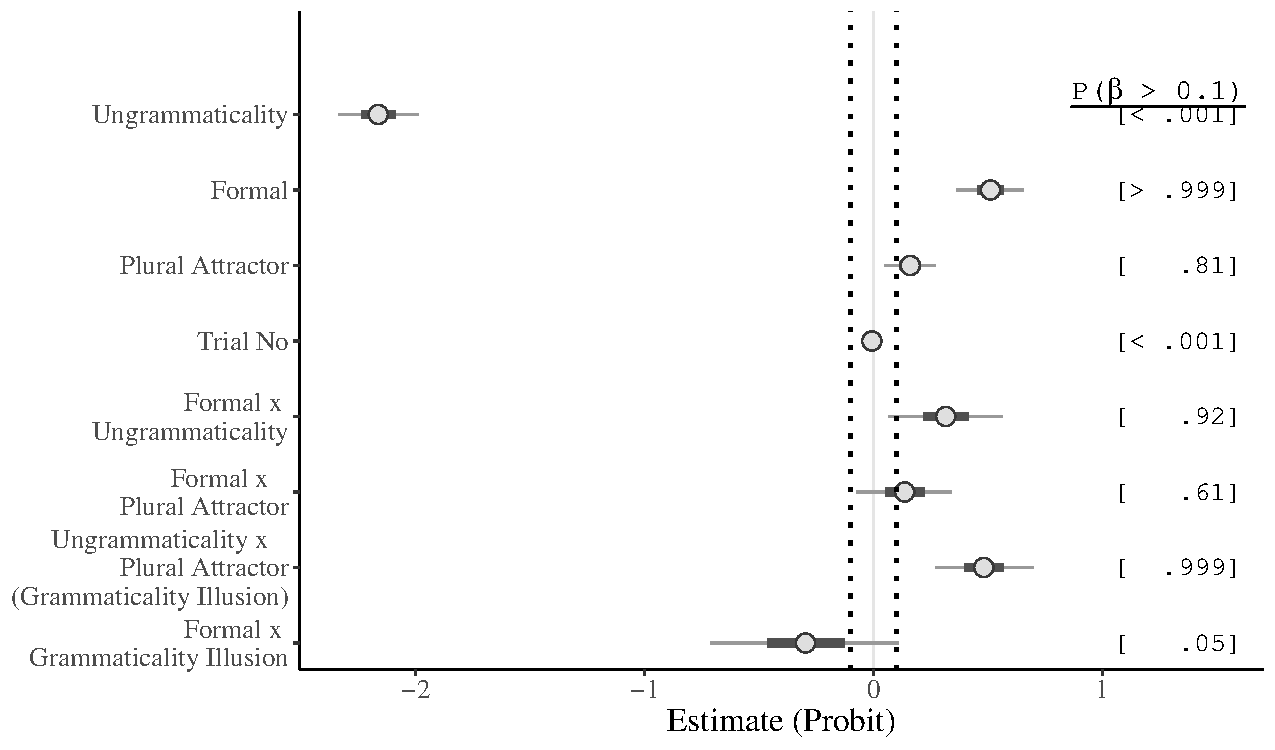
\includegraphics[width=\linewidth]{figure/exp4Bayes-1} 

}

\caption{Estimates and 95\% credible intervals for the probit regression coefficients for the model of responses in our Experiment 4}\label{fig:exp4Bayes}
\end{figure}

\end{knitrout}

The negative main effect of ungrammaticality ($\hat{\beta}=-2.16;$ $CI=[-2.38; -1.96];$ $P(\beta>0.1)< .001$) showed that participants were able to detect ungrammaticality. However, the estimate is smaller than our previous experiments because the formal register occasionally licensed the presence of plural agreement on the verb. The positive main effect of formal register ($\hat{\beta}=0.51;$ $CI=[0.33; 0.69];$ $P(\beta>0.1)> .999$) was expected given that it licenses the plural agreement. The clear positive effect of the interaction between the ungrammaticality and the plural attractor ($\hat{\beta}=0.48;$ $CI=[0.23; 0.75];$ $P(\beta>0.1)  .999$) showed that the percentage of acceptable responses in ungrammatical are amplified when the attractor is plural independent of the register. The weak negative interaction between the formal register, ungrammaticality, and the plural attractor ($\hat{\beta}=-0.30;$ $CI=[-0.79; 0.18];$ $P(\beta>0.1)   .05$) implied that the presence of an interjection that might induce formality decreased the amplification of the percentage of acceptable responses driven by the existence of plural attractor in ungrammatical sentences. 

\section{Discussion}

Experiment 4 investigated an alternative account for Turkish agreement attraction facts: a plural marker at the verb might induce an honorific reading and increase acceptability in ungrammatical sentences similar to the effects seen in attraction studies. We hypothesized that this honorific reading would not be possible with slang interjections like yo, dude, or lan in Turkish. We conducted a speeded acceptability judgment experiment with eight conditions to test this hypothesis. We manipulated the number of the verb (plural x singular), attractor (plural x singular), and the register (formal x informal).

Our results showed that formal interjections like \emph{sir} increased the overall acceptability in ungrammatical sentences, and the effect of plural attractor was present. More importantly, the same effect of plural attractor was also present in informal register with slang interjection endings. Our results were also certified in our Bayesian GLM: positive interaction between the verb plurality and the attractor plurality independent of the register. 

We can say that the initial findings of Turkish agreement attraction were not due to a formal reading licensing the plural verb. However, these results must be taken with caution since the experimental design was sub-optimal.

